\subsection{Предел рекуррентно заданных последовательностей}
Для того чтобы найти пример рекуррентно заданных последовательностей

\textbf{Шаг 1:} Проверить, что последовательность сходится (можно пытаться делать через теорему Вейерштрасса или критерий Коши)

\textbf{Шаг 2:} Найти предел используя арифметику пределов
\subsection{Постоянная Эйлера}

\section{Подпоследовательности}

\begin{definition}
    \textbf{Подпоследовательностью} последовательности $\{a_n\}$ называется последовательность $\{b_k\}$, такая что $b_k = a_{n_k}$, где $n_k$ - строго возрастающая последовательность номеров ($\N$)
\end{definition}

\begin{remark}[Замечание]
    $$ n_k \geq k $$
\end{remark}

\begin{example}
    $ a_n = \sin \frac{\pi n}{2} $

    $ b_k = a_{4k} = \sin 2\pi k \equiv 0$

    $ c_k = a_{4k - 1} = \sin \frac{\pi (4k - 1)}{2} \equiv -1$

    $ d_k = a_{2k + 1} = \sin \frac{\pi (2k + 1)}{2} = (-1)^k  $
\end{example}

\subsection{Частичные пределы}
\begin{definition}
    \textbf{Частичный предел последовательности -} предел подпоследовательности
\end{definition}

\begin{remark}
У какой (ограниченной) последовательности бесконечное число частичных пределов?
\end{remark}
\subsection{Предельные точки} 
\subsection{Свойства частичных пределов}
\newpage
\subsection{Теорема Больцано-Вейерштрасса}

\begin{theorem}
Если $a_n \underset{n \to \infty}{\to} A, \text{ то}\ \forall n_k\ b_k = a_{n_k} \underset{n \to \infty}{\to} A $ 
\end{theorem}

\begin{Proof}
    $$ \forall \eps > 0\ \exists N(\eps)\ \forall n > N(\eps)\ |a_n - A| < \eps $$
    Хотим
    $$ \forall \eps > 0\ \exists K(\eps)\ \forall k > k(\eps)\ |a_{n_k} - A| < \eps $$
    Возьмем $K(\eps) = N(\eps)$
    \[\begin{array}{l}
        \l.
        \begin{array}{l}
            \forall k > N(\eps)\\
            \text{т.к } n_k \geq k
        \end{array}
        \r]
        \l. \Rightarrow \r.
        \l.
        n_k > N(\eps). \text{ Тогда } |a_{n_k} - A| < \eps \text{ истина}
        \r.
    \end{array}\]
\end{Proof}

\begin{figure}[h]
  \centering
  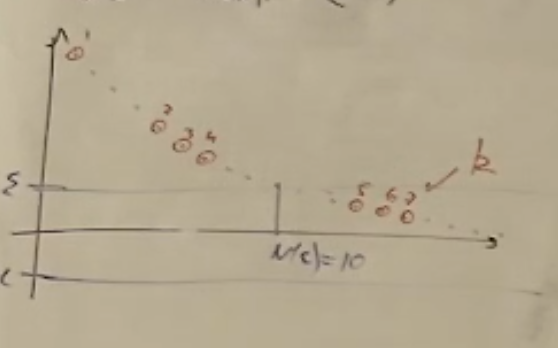
\includegraphics[width=0.5\textwidth]{lectures/files/lec_6_10.10.2025-19-24-42.png}
  \caption{К теореме}
  \label{fig:lec_6_10.10.2025-19-24-42.png}
\end{figure}

\begin{theorem}[Теорема Больцано-Вейерштрасса]
    Если последовательность ограничена, то у нее есть сходящаяся подпоследовательность
\end{theorem}

\begin{Proof}
    $c_n$ -- огр. Докажем что у нее есть сходящаяся подпоследовательность

    $A = inf\{c_n\}$
    
    $B = sup\{c_n\}$

    $A, B \in \R$

    Рассмотрим отрезок $[a_1,b_1] = [A,B]$

    \textbf{Шаг 1:} разделим отрезок $[a_1,b_1]$ пополам. В какой-то половине (одной или обеих) лежит бесконечное число членов $c_n$. Выберем в качестве $[a_2,b_2]$ эту половинку (если в обеих бесконечное число, то любую)

    \textbf{Шаг 2:} $\ldots$

    Получаем некоторую последовательность подотрезков $\{[a_k,b_k]\}_{k \in \N}$

    На первом шаге выберем какой-то член $c_n \in [a_1,b_1]$. Его номер возьмем в качестве~$n_1$

    $\exists$ член последовательности $\in [a_2,b_2]$ такой, что его номер $> n_1$ (Это следует из того, что на каждом шаге мы выбираем отрезок, содержащий бесконечное число членов). Его возьмем в качестве $n_2$

    $\ldots$

    Таким образом, параллельно строя последовательность отрезков, мы построили подпоследовательность $\{C_{n_k}\}_{k\in\N}$

    Рассмотрим $\{a_k\}_{k\in\N}$. Она неубывает, ограничена сверху $B$. \\По т. Вейерштрасса: $\exists \Lim{k}{\infty} a_k = A'$

    $\{b_k\}_{k\in\N}$. Она невозрастает, ограничена снизу $A$. \\По т. Вейерштрасса: $\exists \Lim{k}{\infty} b_k = B'$

    На каждом шаге мы вдвое уменьшаем длину отрезка. Выпишем общую формулу:
    
    // TODO
    $$ b_k - a_k $$
\end{Proof}

\begin{example}
    $c_n = (-1)^n$
\end{example}

\begin{figure}[h]
\centering
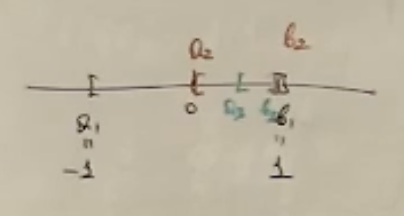
\includegraphics[width=0.5\textwidth]{lectures/files/lec6-21-17-51.png}
\caption{К примеру}
\label{fig:lec6-21-17-51.png}
\end{figure}

\subsection{Критерий Коши}
